%\PassOptionsToPackage{landscape}{geometry}
\documentclass[aspectratio=169]{beamer}

%\input{nonLightBoard_slides.tex}
\usepackage{bm}

%\usepackage{graphics}
\usepackage{graphicx}
\usepackage{amsmath,amssymb,amsthm}
\usepackage{bm}
%\usepackage{subfigure}

\usepackage{xcolor}
\usepackage{colortbl}

\def\boldred#1{\color{red}\textbf{#1}}

\def\IC{\mathbb{C}}
\def\IF{\mathbb{F}}
\def\II{\mathbb{I}}
\def\IM{\mathbb{M}}
\def\IN{\mathbb{N}}
\def\IP{\mathbb{P}}
\def\IR{\mathbb{R}}
\def\IZ{\mathbb{Z}}

\def\ba{\mathbf{a}}
\def\bb{\mathbf{b}}
\def\bc{\mathbf{c}}
\def\be{\mathbf{e}}
\def\bg{\mathbf{g}}
\def\bh{\mathbf{h}}
\def\bi{\mathbf{i}}
\def\bj{\mathbf{j}}
\def\bk{\mathbf{k}}
\def\bn{\mathbf{n}}
\def\bp{\mathbf{p}}
\def\br{\mathbf{r}}
\def\bs{\mathbf{s}}
\def\bu{\mathbf{u}}
\def\bv{\mathbf{v}}
\def\bw{\mathbf{w}}
\def\bx{\mathbf{x}}
\def\by{\mathbf{y}}
\def\bz{\mathbf{z}}

\def\bB{\mathbf{B}}
\def\bD{\mathbf{D}}
\def\bF{\mathbf{F}}
\def\bG{\mathbf{G}}
\def\bN{\mathbf{N}}
\def\bR{\mathbf{R}}
\def\bS{\mathbf{S}}
\def\bT{\mathbf{T}}
\def\b0{\mathbf{0}}

\bmdefine{\bmu}{\bm{\mu}}

\def\A{\mathcal{A}}
\def\B{\mathcal{B}}
\def\C{\mathcal{C}}
\def\D{\mathcal{D}}
\def\E{\mathcal{E}}
\def\F{\mathcal{F}}
\def\G{\mathcal{G}}
\def\I{\mathcal{I}}
\def\L{\mathcal{L}}
\def\M{\mathcal{M}}
\def\N{\mathcal{N}}
\def\P{\mathcal{P}}
\def\R{\mathcal{R}}
\def\S{\mathcal{S}}
\def\T{\mathcal{T}}
\def\U{\mathcal{U}}
\def\V{\mathcal{V}}

\def\nbOne{{\mathchoice {\rm 1\mskip-4mu l} {\rm 1\mskip-4mu l}
{\rm 1\mskip-4.5mu l} {\rm 1\mskip-5mu l}}}

\def\cov{\ensuremath{\mathsf{cov}}}
\def\Var{\ensuremath{\mathsf{Var}\ }}

\def\defword#1{\textbf{#1}\index{#1}}



%%%%%%%%%%%%%%%%%%%%%
%%%%%%%%%%%%%%%%%%%%%
%%
%%
%% NAVIGATION AND SECTIONING
%%
%%
%%%%%%%%%%%%%%%%%%%%%
%%%%%%%%%%%%%%%%%%%%%
\def\sgn{\ensuremath{\mathsf{sgn}}}

\newtheorem{proposition}[theorem]{Proposition}
\newtheorem{property}[theorem]{Property}
\newtheorem{importantproperty}[theorem]{Property}
\newtheorem{importanttheorem}[theorem]{Theorem}
%\newtheorem{lemma}[theorem]{Lemma}



\setbeamertemplate{navigation symbols}{}
\setbeamertemplate{footline}
{%
	\quad\insertsection\hfill p. \insertpagenumber\quad\mbox{}\vskip2pt
}
\usecolortheme{orchid}
\setbeamertemplate{theorems}[numbered]

\makeatletter
\newlength\beamerleftmargin
\setlength\beamerleftmargin{\Gm@lmargin}
\makeatother

%%%%%%%%%%%
% To have links to parts in the outline
\makeatletter
\AtBeginPart{%
	\addtocontents{toc}{\protect\beamer@partintoc{\the\c@part}{\beamer@partnameshort}{\the\c@page}}%
}
%% number, shortname, page.
\providecommand\beamer@partintoc[3]{%
	\ifnum\c@tocdepth=-1\relax
	% requesting onlyparts.
	\makebox[6em]{Chapter #1:} \textcolor{green!30!blue}{\hyperlink{#2}{#2}}
	\par
	\fi
}
\define@key{beamertoc}{onlyparts}[]{%
	\c@tocdepth=-1\relax
}
\makeatother%

\newcommand{\nameofthepart}{}
\newcommand{\nupart}[1]%
{   \part{#1}%
	\renewcommand{\nameofthepart}{#1}%
	{
		\setbeamercolor{background canvas}{bg=orange!50}
		\begin{frame}{#1}%\partpage 
			\hypertarget{\nameofthepart}{}\tableofcontents%
		\end{frame}
	}
}

% Beginning of a section
\AtBeginSection[]{
	{
		\setbeamercolor{background canvas}{bg=orange!10}
		\begin{frame}[noframenumbering,plain]
			\tableofcontents[currentsection,hideothersubsections]
		\end{frame}
		\addtocounter{page}{-1}
		%\addtocounter{framenumber}{-1} 
	}
}

% Beginning of a section
\AtBeginSubsection[]{
	{
		\setbeamercolor{background canvas}{bg=orange!10}
		\begin{frame}[noframenumbering,plain]
			\tableofcontents[sectionstyle=show/shaded,subsectionstyle=show/shaded/hide]
		\end{frame}
		\addtocounter{page}{-1}
		%\addtocounter{framenumber}{-1} 
	}
}




%%%%%%%%%%%%%%%%%%%%%
%%%%%%%%%%%%%%%%%%%%%
%%
%%
%% COLOURED ENVIRONMENTS
%%
%%
%%%%%%%%%%%%%%%%%%%%%
%%%%%%%%%%%%%%%%%%%%%
% \newtheorem{proposition}[theorem]{Proposition}
% \newtheorem{property}[theorem]{Property}
% \newtheorem{importantproperty}[theorem]{Property}
% \newtheorem{importanttheorem}[theorem]{Theorem}
%\newtheorem{lemma}[theorem]{Lemma}
%%%%%%% 
%% Definitions in yellow boxes
\usepackage{etoolbox}
\setbeamercolor{block title}{use=structure,fg=structure.fg,bg=structure.fg!05!bg}
\setbeamercolor{block body}{parent=normal text,use=block title,bg=block title.bg!20!bg}

\BeforeBeginEnvironment{definition}{%
	\setbeamercolor{block title}{fg=black,bg=yellow!20!white}
	\setbeamercolor{block body}{fg=black, bg=yellow!05!white}
}
\AfterEndEnvironment{definition}{
	\setbeamercolor{block title}{use=structure,fg=structure.fg,bg=structure.fg!20!bg}
	\setbeamercolor{block body}{parent=normal text,use=block title,bg=block title.bg!50!bg, fg=black}
}
\BeforeBeginEnvironment{importanttheorem}{%
	\setbeamercolor{block title}{fg=black,bg=red!20!white}
	\setbeamercolor{block body}{fg=black, bg=red!05!white}
}
\AfterEndEnvironment{importanttheorem}{
	\setbeamercolor{block title}{use=structure,fg=structure.fg,bg=structure.fg!20!bg}
	\setbeamercolor{block body}{parent=normal text,use=block title,bg=block title.bg!50!bg, fg=black}
}
\BeforeBeginEnvironment{importantproperty}{%
	\setbeamercolor{block title}{fg=black,bg=red!50!white}
	\setbeamercolor{block body}{fg=black, bg=red!30!white}
}
\AfterEndEnvironment{importantproperty}{
	\setbeamercolor{block title}{use=structure,fg=structure.fg,bg=structure.fg!20!bg}
	\setbeamercolor{block body}{parent=normal text,use=block title,bg=block title.bg!50!bg, fg=black}
}


% Colours for special pages
\def\extraContent{yellow!20}

% Allow to change slide colour
% From: https://tex.stackexchange.com/questions/8043/change-the-background-color-of-a-frame-in-beamer
\defbeamertemplate*{background canvas}{mydefault}{%
	\ifbeamercolorempty[bg]{background canvas}{}{\color{bg}\vrule width\paperwidth height\paperheight}% copied beamer default here
}
\defbeamertemplate*{background canvas}{bg}{%
	\color{lightgray!20}\vrule width\paperwidth height\paperheight% added bg color
}
\BeforeBeginEnvironment{frame}{%
	\setbeamertemplate{background canvas}[mydefault]%
}
\makeatletter
\define@key{beamerframe}{bg}[true]{%
	\setbeamertemplate{background canvas}[bg]%
}
\makeatother
% Use with
%\begin{frame}
% \frametitle{Normal}
%\end{frame} 
%\begin{frame}[bg]
% \frametitle{With bg}
%\end{frame}


% Vertical alignment on pages
% From: https://tex.stackexchange.com/questions/148365/how-do-i-ask-beamer-to-exactly-fill-up-a-slide
% Turn on with
% \stretchon
% (outside slide), and off with
% \stretchoff
\def\itemsymbol{$\blacktriangleright$}
%\def\itemsymbol{}
\let\svpar\par
\let\svitemize\itemize
\let\svenditemize\enditemize
\let\svitem\item
\let\svcenter\center
\let\svendcenter\endcenter
\let\svcolumn\column
\let\svendcolumn\endcolumn
\def\newitem{\renewcommand\item[1][\itemsymbol]{\vfill\svitem[##1]}}%
\def\newpar{\def\par{\svpar\vfill}}%
\newcommand\stretchon{%
	\newpar%
	\renewcommand\item[1][\itemsymbol]{\svitem[##1]\newitem}%
	\renewenvironment{itemize}%
	{\svitemize}{\svenditemize\newpar\par}%
	\renewenvironment{center}%
	{\svcenter\newpar}{\svendcenter\newpar}%
	\renewenvironment{column}[2]%
	{\svcolumn{##1}\setlength{\parskip}{\columnskip}##2}%
	{\svendcolumn\vspace{\columnskip}}%
}
\newcommand\stretchoff{%
	\let\par\svpar%
	\let\item\svitem%
	\let\itemize\svitemize%
	\let\enditemize\svenditemize%
	\let\center\svcenter%
	\let\endcenter\svendcenter%
	\let\column\svcolumn%
	\let\endcolumn\svendcolumn%
}
\newlength\columnskip
\columnskip 0pt

%%%%%%%%%%%%%%%%%
\usepackage{tikz}
\usetikzlibrary{shapes,arrows}
\usetikzlibrary{positioning}
\tikzstyle{cloud} = [draw, ellipse,fill=red!20, node distance=0.87cm,
minimum height=2em]
\tikzstyle{line} = [draw, -latex']
\usetikzlibrary{shapes.symbols,shapes.callouts,patterns}
\usetikzlibrary{calc,fit}
\usetikzlibrary{backgrounds}

\usetikzlibrary{decorations.pathmorphing,backgrounds,positioning,fit,petri}
\usetikzlibrary{automata}

% Index in the slides as well
\usepackage{makeidx}
\makeindex
\newenvironment{theindex}
 {\let\item\par
  %definitions for subitem etc
  }{}
\newcommand\indexspace{}

% Beginning of a section
\AtBeginSection[]{
	{
		\setbeamercolor{background canvas}{bg=orange!10}
		\begin{frame}[noframenumbering,plain]
			\framesubtitle{\nameofthepart Chapter \insertromanpartnumber \ -- \iteminsert{\insertpart}}
			\tableofcontents[currentsection,currentsubsection]
		\end{frame}
	\addtocounter{page}{-1}
	%\addtocounter{framenumber}{-1} 
	}
}


\title{Clustering \& Classification}
\date{}

\begin{document}
\DeclareFontShape{OT1}{cmss}{b}{n}{<->ssub * cmss/bx/n}{} 
\begin{frame}
	\titlepage
\end{frame}

%%%%%%%%%%%%%%%%%%%
%%%%%%%%%%%%%%%%%%%
%%%%%%%%%%%%%%%%%%%
%%%%%%%%%%%%%%%%%%%
\section{What are clustering and classification ?}

\begin{frame}{Clustering vs classification}
    Clustering is partitioning an unlabelled dataset into groups of similar objects
    \vfill
    Classification sorts data into specific categories using a labelled dataset
\end{frame}

\begin{frame}{Clustering}
    From \href{https://en.wikipedia.org/wiki/Cluster_analysis}{Wikipedia}
    \begin{quote}
        \textbf{Cluster analysis} or \textbf{clustering} is the task of grouping a set of objects in such a way that objects in the same group (called a \textbf{cluster}) are more similar (in some sense) to each other than to those in other groups (clusters).
    \end{quote}
    \vfill
    There are a myriad of ways to do clustering, this is an extremely active field of research and application. See the Wikipedia page for leads
\end{frame}


\begin{frame}{We have done clustering already}
    We have seen some clustering:
    \begin{itemize}
        \item when we sought strongly connected components
        \item when we sought cliques
        \item to some extent, with PCA
    \end{itemize}   
\end{frame}


\begin{frame}{Classification}
    From \href{https://en.wikipedia.org/wiki/Statistical_classification}{Wikipedia}
    \begin{quote}
        In statistics, \textbf{classification} is the problem of identifying which of a set of categories (sub-populations) an observation (or observations) belongs to. Examples are assigning a given email to the "spam" or "non-spam" class, and assigning a diagnosis to a given patient based on observed characteristics of the patient (sex, blood pressure, presence or absence of certain symptoms, etc.).
    \end{quote}
\end{frame}

%%%%%%%%%%%%%%%%%%%
%%%%%%%%%%%%%%%%%%%
%%%%%%%%%%%%%%%%%%%
%%%%%%%%%%%%%%%%%%%
\section{Support vector machines}

\begin{frame}{Support vector machines (SVM)}
    We are given a training dataset of $n$ points of the form
    \[ 
        (\bx_1, y_1), \ldots, (\bx_n, y_n)
    \]
    where $\bx_i\in\IR^p$ and $y_i=\{-1,1\}$. The value of $y_i$ indicates the class to which the point $\bx_i $ belongs
    \vfill
    We want to find a \textbf{surface} $\S$ in $\IR^p$ that divides the group of points into two subgroups
    \vfill
    Once we have this surface $\S$, any additional point that is added to the set can then be \emph{classified} as belonging to either one of the sets depending on where it is with respect to the surface $\S$
\end{frame}

\begin{frame}{Linear SVM}
    We are given a training dataset of $n$ points of the form
    \[ 
        (\bx_1, y_1), \ldots, (\bx_n, y_n)
    \]
    where $\bx_i\in\IR^p$ and $y_i=\{-1,1\}$. The value of $y_i$ indicates the class to which the point $\bx_i $ belongs
    \vfill
    \begin{quote}\textbf{Linear SVM --}
        Find the ``maximum-margin hyperplane'' that divides the group of points $\bx_i$ for which $y_i = 1$ from the group of points for which $y_i = -1$, which is such that the distance between the hyperplane and the nearest point $\bx_i$ from either group is maximized.
    \end{quote}
\end{frame}

\begin{frame}
    \begin{minipage}{0.7\textwidth}
        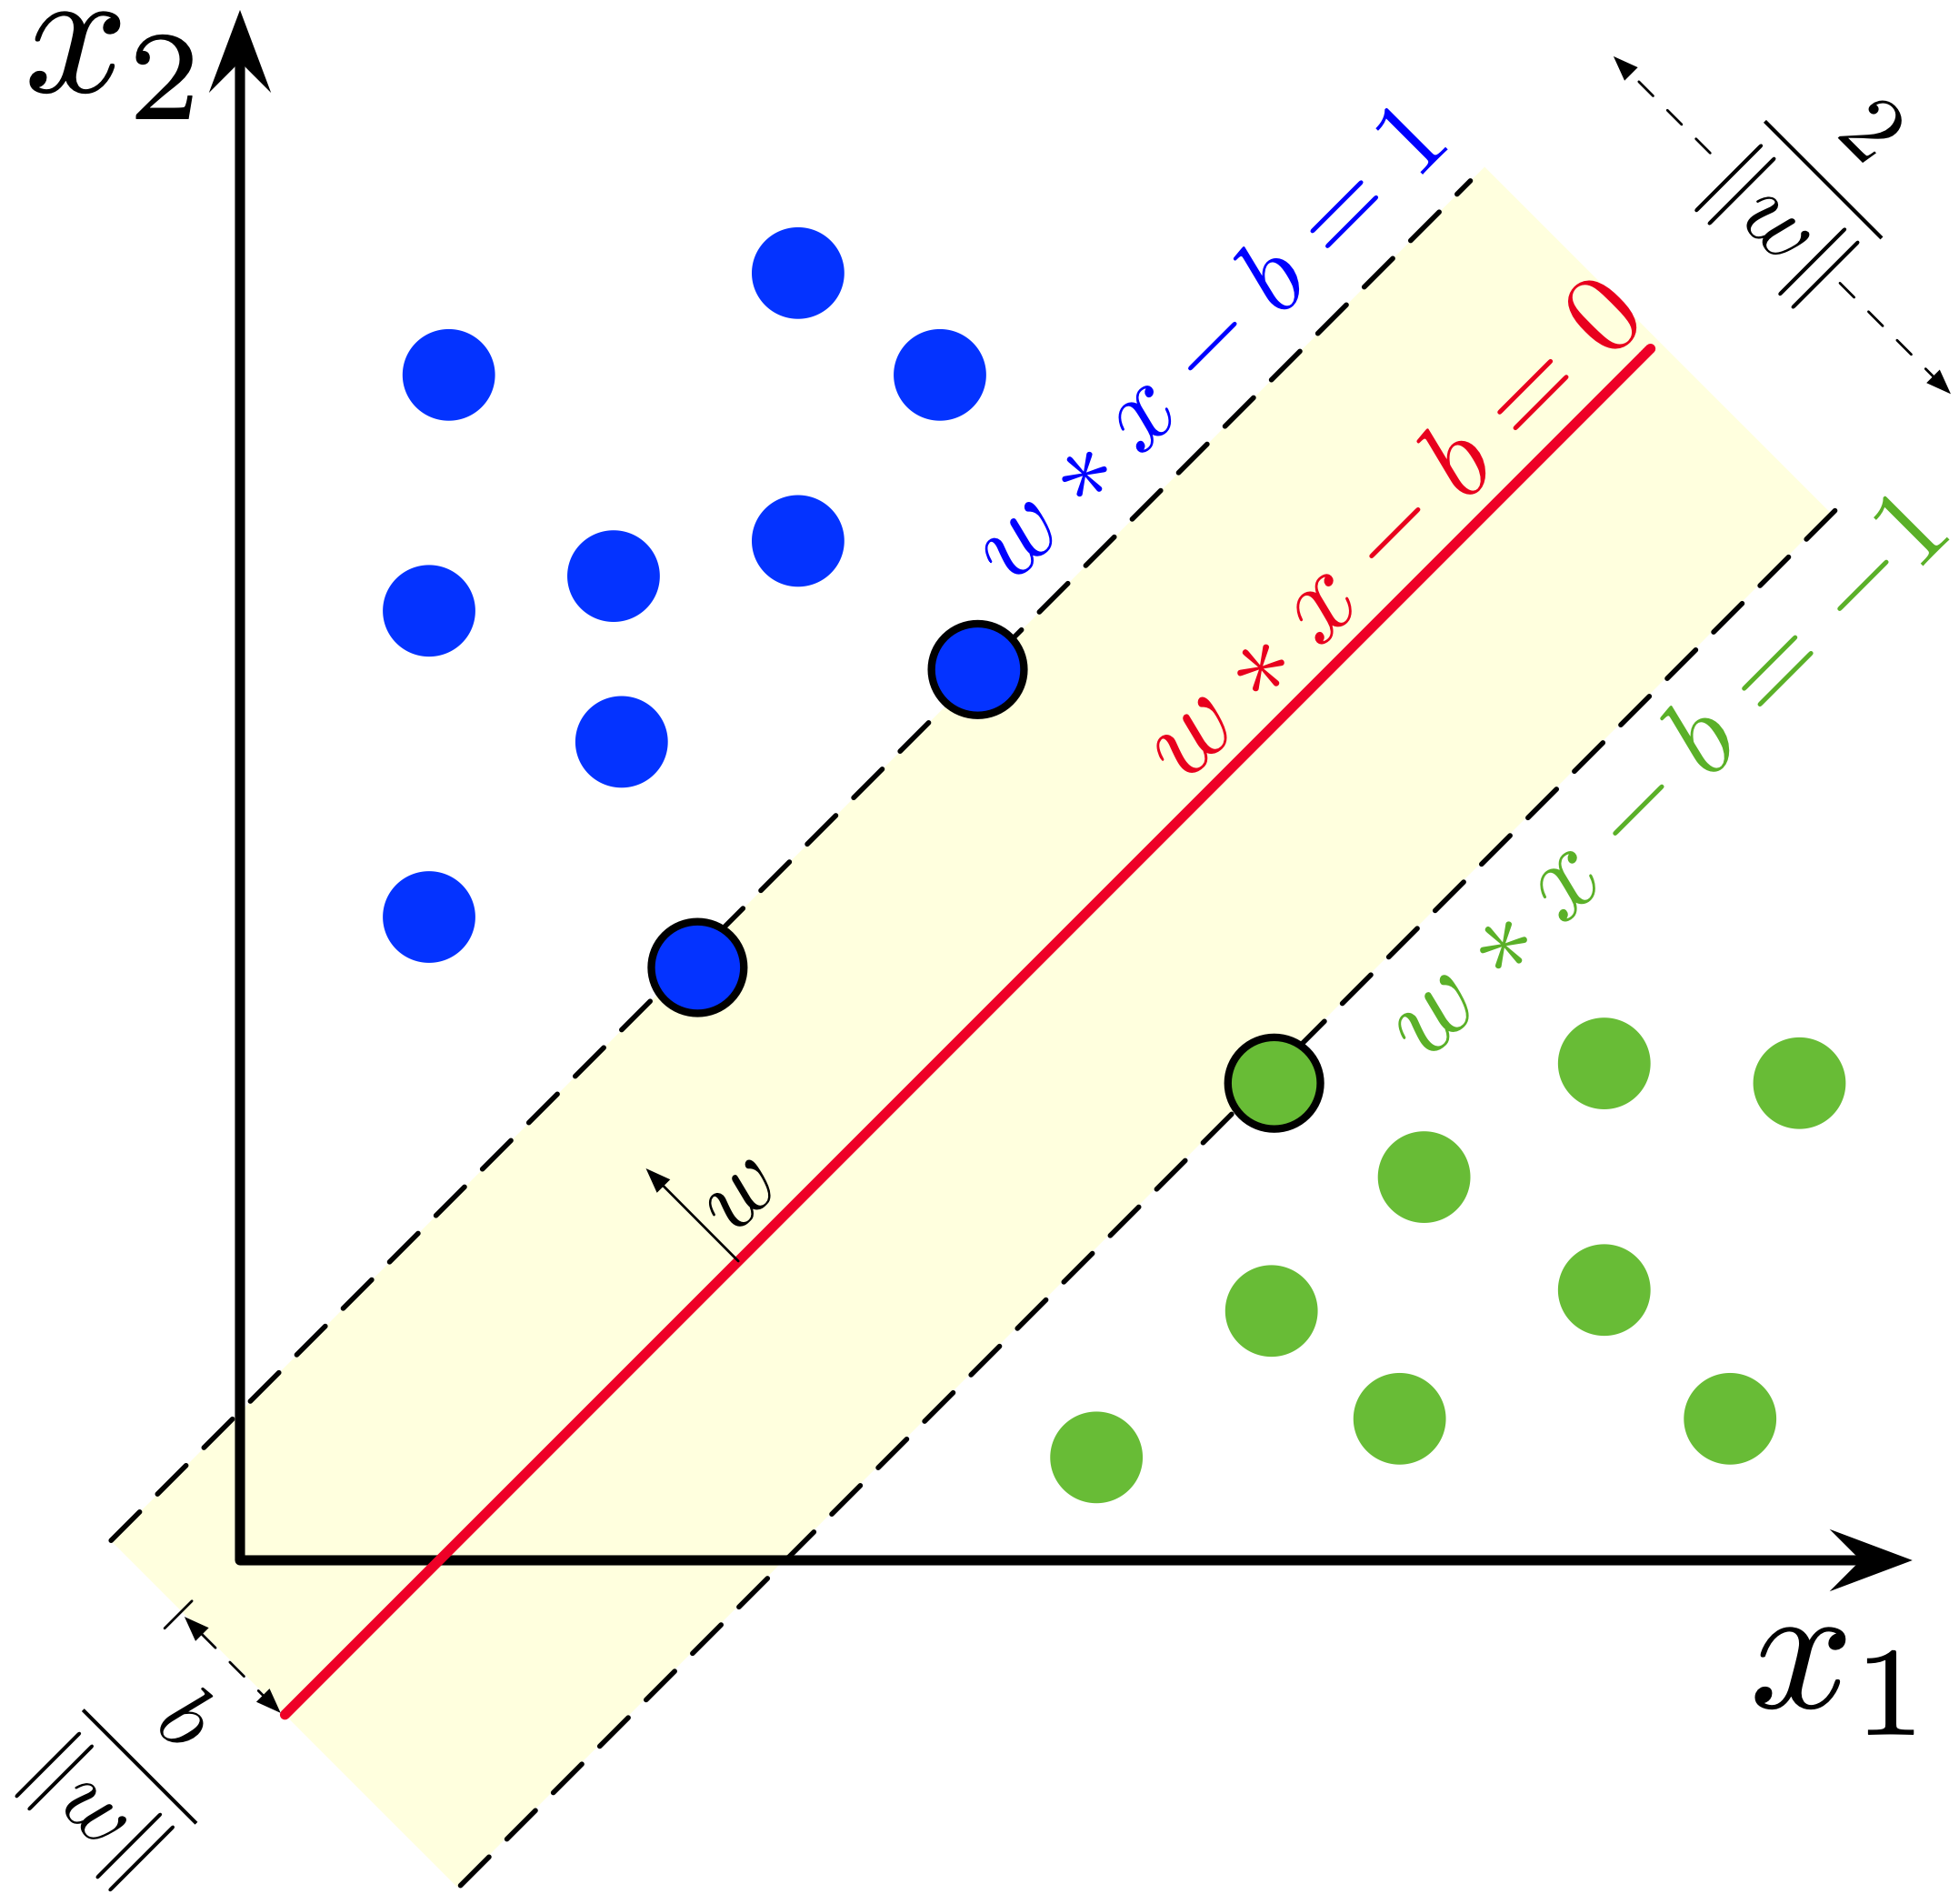
\includegraphics[height=\textheight]{FIGS_slides/SVM_margin}
    \end{minipage}
    \begin{minipage}{0.28\textwidth}
        Maximum-margin hyperplane and margins for an SVM trained with samples from two classes. Samples on the margin are the \textbf{support vectors}
    \end{minipage}
\end{frame}

\begin{frame}
    Any \textbf{hyperplane} can be written as the set of points $\mathbf{x}$ satisfying
    \[
        \bw^\mathsf{T} \bx - b = 0
    \]
    where $\bw$ is the (not necessarily normalized) \textbf{normal vector} to the hyperplane (if the hyperplane has equation $a_1z_1+\cdots+a_pz_p=c$, then $(a_1,\ldots,a_n)$ is normal to the hyperplane)
    % \vfill
    % This is much like \textbf{Hesse normal form}, except that $\mathbf{w}$ is not necessarily a unit vector
    \vfill
    The parameter $b/\|\bw\|$ determines the offset of the hyperplane from the origin along the normal vector $\bw$
    \vfill
    Remark: a hyperplane defined thusly is not a subspace of $\IR^p$ unless $b=0$. We can of course transform the data so that it is...
\end{frame}

\begin{frame}{Linearly separable points}
    Let $X_1$ and $X_2$ be two sets of points in $\IR^p$ 
    \vfill
    Then $X_1$ and $X_2$ are \textbf{linearly separable} if there exist $w_{1}, w_{2},..,w_{p}, k\in\IR$ such that 
    \begin{itemize}
        \item every point $x \in X_1$ satisfies $\sum^{p}_{i=1} w_{i}x_{i} > k$ 
        \item every point $x \in X_2$ satisfies $\sum^{p}_{i=1} w_{i}x_{i} < k$
    \end{itemize}
    where $x_{i}$ is the $i$th component of $x$
\end{frame}

\begin{frame}{Hard-margin SVM}
    If the training data is \textbf{linearly separable}, we can select two parallel hyperplanes that separate the two classes of data, so that the distance between them is as large as possible 
    \vfill
    The region bounded by these two hyperplanes is called the ``margin'', and the maximum-margin hyperplane is the hyperplane that lies halfway between them
    \vfill
    With a normalized or standardized dataset, these hyperplanes can be described by the equations
    \begin{itemize}
        \item $\mathbf{w}^\mathsf{T} \mathbf{x} - b = 1$ (anything on or above this boundary is of one class, with label 1) 
        \item $\mathbf{w}^\mathsf{T} \mathbf{x} - b = -1$ (anything on or below this boundary is of the other class, with label -1)
    \end{itemize}
\end{frame}

\begin{frame}
    Distance between these two hyperplanes is $2/\|\bw\|$
    \vfill
    $\Rightarrow$ to maximize the distance between the planes we want to minimize $\|\bw\|$
    \vfill
    The distance is computed using the distance from a point to a plane equation
    \vfill
    We must also prevent data points from falling into the margin, so we add the following constraint: for each $i$ either
    \[
        \mathbf{w}^\mathsf{T} \mathbf{x}_i - b \ge 1 \, , \text{ if } y_i = 1
    \]
    or
    \[
        \mathbf{w}^\mathsf{T} \mathbf{x}_i - b \le -1 \, , \text{ if } y_i = -1
    \]
    \vfill
    (Each data point must lie on the correct side of the margin)
\end{frame}

\begin{frame}
    This can be rewritten as
    \[
        y_i(\mathbf{w}^\mathsf{T} \mathbf{x}_i - b) \ge 1, \quad \text{ for all } 1 \le i \le n
    \]
    or
    \[
        y_i(\mathbf{w}^\mathsf{T} \mathbf{x}_i - b)-1\geq 0, \quad \text{ for all } 1 \le i \le n
    \]
    \vfill
    We get the optimization problem:
    \begin{quote}
        Minimize $\|\mathbf{w}\|$ subject to $y_i(\mathbf{w}^\mathsf{T} \mathbf{x}_i - b)-1 \ge 0$ for $i = 1, \ldots, n$
    \end{quote}
    \vfill
    The $\mathbf{w}$ and $b$ that solve this problem determine the classifier, $\mathbf{x} \mapsto \sgn(\mathbf{w}^\mathsf{T} \mathbf{x} - b)$ where $\sgn(\cdot)$ is the \textbf{sign function}.
\end{frame}

\begin{frame}   
    The maximum-margin hyperplane is completely determined by those $\bx_i$ that lie nearest to it
    \vfill
    These $\bx_i$ are the \textbf{support vectors}
\end{frame}

\begin{frame}{Writing the goal in terms of Lagrange multipliers}
    Recall that our goal is to
    \begin{quote}
        minimize $\|\mathbf{w}\|$ subject to $y_i(\mathbf{w}^\mathsf{T} \mathbf{x}_i - b)-1 \ge 0$ for $i = 1, \ldots, n$
    \end{quote}
    \vfill
    Using Lagrange multipliers $\lambda_1,\ldots,\lambda_n$, we have the function
    \[
        L_P:=F(\bw,b\lambda_1,\ldots,\lambda_n) =
        \frac 12\|\bw\|^2 -\sum_{i=1}^n \lambda_iy_i(\bx_i\bw+b)
        +\sum_{i=1}^n\lambda_i
    \]
    \vfill
    Note that we have as many Lagrange multipliers as there are data points. Indeed, there are that many inequalities that must be satisfied
    \vfill 
    The aim is to minimise $L_p$ with respect to $\bw$ and $b$ while the derivatives of $L_p$ w.r.t. $\lambda_i$ vanish and the $\lambda_i\geq 0$, $i=1,\ldots,n$
\end{frame}

\begin{frame}{Lagrange multipliers}
    We have already seen Lagrange multipliers, when we were studying PCA
    \vfill
\end{frame}

\begin{frame}{Maximisation using Lagrange multipliers (V1.0)}
    We want the max of $f(x_1,\ldots,x_n)$ under the constraint $g(x_1,\ldots,x_n)=k$
    \begin{enumerate}
    \item Solve
    \begin{align*}
    \nabla f(x_1,\ldots,x_n) &= \lambda\nabla g(x_1,\ldots,x_n) \\
    g(x_1,\ldots,x_n) &= k
    \end{align*}
    where $\nabla=(\frac{\partial}{\partial x_1},\ldots,\frac{\partial}{\partial x_n})$ is the \textbf{gradient operator}
    \item Plug all solutions into $f(x_1,\ldots,x_n)$ and find maximum values (provided values exist and $\nabla g\neq \b0$ there)
    \end{enumerate}
    \vfill
    $\lambda$ is the \textbf{Lagrange multiplier}
\end{frame}
    
    
\begin{frame}{The gradient}
    $f:\IR^n\to\IR$ function of several variables, $\nabla=\left(\frac{\partial}{\partial x_1},\ldots,\frac{\partial}{\partial x_n}\right)$ the gradient operator
    \vfill
    Then
    \[
    \nabla f = \left(
    \frac{\partial}{\partial x_1}f,\ldots,
    \frac{\partial}{\partial x_n}f
    \right)
    \]
    \vfill
    So $\nabla f$ is a \emph{vector-valued} function, $\nabla f:\IR^n\to\IR^n$; also written as
    \[
    \nabla f = f_{x_1}(x_1,\ldots,x_n)\be_1+\cdots f_{x_n}(x_1,\ldots,x_n)\be_n
    \]
    where $f_{x_i}$ is the partial derivative of $f$ with respect to $x_i$ and $\{\be_1,\ldots,\be_n\}$ is the standard basis of $\IR^n$
\end{frame}

\begin{frame}{Lagrange multipliers (V2.0)}
        However, the problem we were considering then involved a single multiplier $\lambda$
        \vfill
        Here we want $\lambda_1,\ldots,\lambda_n$
\end{frame}

\begin{frame}{Lagrange multiplier theorem}
    \begin{theorem}
        Let $f\colon\mathbb{R}^n \rightarrow \mathbb{R}$ be the objective function, $g\colon\mathbb{R}^n \rightarrow \mathbb{R}^c $ be the constraints function, both being $C^1$.
        Consider the optimisation problem
        \begin{align*}
            \text{maximize}\ f(x) \\
            \text{subject to}\ g(x) = 0                 
        \end{align*}
        Let $x^*$ be an optimal solution to the optimization problem, such that $\operatorname{rank} (Dg(x^*)) = c < n$, where $Dg(x^*)$ denotes the matrix of partial derivatives
        \[
            \left[{\partial g_j}/{\partial x_k}\right]  
        \]
        Then there exists a unique Lagrange multiplier $\lambda^* \in \mathbb{R}^c$ such that
        \[
            Df(x^*) = \lambda^{*T}Dg(x^*)
        \]
    \end{theorem}
\end{frame}

\begin{frame}{Lagrange multipliers (V3.0)}
    Here we want $\lambda_1,\ldots,\lambda_n$
    \vfill
    But we also are looking for $\lambda_i\geq 0$
    \vfill 
    So we need to consider the so-called Karush-Kuhn-Tucker (KKT) conditions
\end{frame}

\begin{frame}{Karush-Kuhn-Tucker (KKT) conditions}
    Consider the optimisation problem
    \begin{align*}
        \text{maximize}\ f(x) \\
        \text{subject to}& \quad g_i(x) \leq 0  \\
        &\quad h_i(x)=0               
    \end{align*}
    Form the Lagrangian
    \[
        L(\bx,\mu,\lambda) = f(\bx)+\mu^T\bg(\bx)+\lambda^T\bh(\bx)
    \]
    \begin{theorem}
        If $(\mathbf{x}^{\ast},\mathbf{\mu}^\ast)$ is a \emph{saddle point} of $L(\mathbf{x},\mathbf{\mu})$ in $\mathbf{x} \in \mathbf{X}$, $\mathbf{\mu} \geq \mathbf{0}$, then $\mathbf{x}^{\ast}$ is an optimal vector for the above optimization problem. Suppose that $f(\mathbf{x})$ and $g_i(\mathbf{x})$, $i = 1, \ldots, m$, are \emph{convex} in $\mathbf{x}$ and that there exists $\mathbf{x}_{0} \in \mathbf{X}$ such that $\mathbf{g}(\mathbf{x}_{0}) < 0$. Then with an optimal vector $\mathbf{x}^{\ast}$ for the above optimization problem there is associated a non-negative vector $\mathbf{\mu}^\ast$ such that $L(\mathbf{x}^{\ast},\mathbf{\mu}^\ast)$ is a saddle point of $L(\mathbf{x},\mathbf{\mu})$
    \end{theorem}
\end{frame}

\begin{frame}{KKT conditions}
    \begin{align*}
        \frac{\partial}{\partial w_\nu}L_P &=
        w_\nu-\sum_{i}^n\lambda_iy_ix_{i\nu}=0
        \qquad\nu=1,\ldots,p \\
        \frac{\partial}{\partial b}L_P &=
        -\sum_{i=1}^n \lambda_iy_i = 0 \\
        y_i(\bx_i^T\bw+b)-1 &\geq 0\qquad i=1,\ldots,n \\
        \lambda_i &\geq 0\qquad i=1,\ldots,n \\
        \lambda_i(y_i(\bx_i^T\bw+b)-1) &=0\qquad i=1,\ldots,n \\
    \end{align*}
\end{frame}


    
\begin{frame}{Soft-margin SVM}
    To extend SVM to cases in which the data are not linearly separable, the \textbf{hinge loss} function is helpful
    \[
        \max\left(0, 1 - y_i(\mathbf{w}^\mathsf{T} \mathbf{x}_i - b)\right)
    \]
    \vfill
    $y_i$ is the $i$th target (i.e., in this case, 1 or -1), and $\mathbf{w}^\mathsf{T} \mathbf{x}_i - b$ is the $i$-th output
    \vfill
    This function is zero if the constraint is satisfied, in other words, if $\mathbf{x}_i$ lies on the correct side of the margin
    \vfill 
    For data on the wrong side of the margin, the function's value is proportional to the distance from the margin
\end{frame}

\begin{frame}
   
    The goal of the optimization then is to minimize
    
    \[ 
        \lambda \lVert \mathbf{w} \rVert^2 +\left[\frac 1 n \sum_{i=1}^n \max\left(0, 1 - y_i(\mathbf{w}^\mathsf{T} \mathbf{x}_i - b)\right) \right]
    \]
    
    where the parameter $\lambda > 0$ determines the trade-off between increasing the margin size and ensuring that the $\mathbf{x}_i$ lie on the correct side of the margin
    \vfill
    Thus, for sufficiently small values of $\lambda$, it will behave similar to the hard-margin SVM, if the input data are linearly classifiable, but will still learn if a classification rule is viable or not
\end{frame}

%%%%%%%%%%%%%%%%%%%
%%%%%%%%%%%%%%%%%%%
%%%%%%%%%%%%%%%%%%%
%%%%%%%%%%%%%%%%%%%
\section{Neural networks (the perceptron)}

\begin{frame}{Artificial neural network (ANN) - from \href{https://en.wikipedia.org/wiki/Artificial_neural_network}{Wikipedia}}
    \begin{quote}
    \textbf{Artificial neural networks} (ANNs) are computing systems inspired by the biological neural networks that constitute animal brains
    \vfill
    An ANN is based on a collection of connected units or nodes called \textbf{artificial neurons}, which loosely model the neurons in a biological brain. Each connection, like the synapses in a biological brain, can transmit a signal to other neurons. An artificial neuron receives signals then processes them and can signal neurons connected to it. The ``signal" at a connection is a real number, and the output of each neuron is computed by some non-linear function of the sum of its inputs. The connections are called edges. Neurons and edges typically have a weight that adjusts as learning proceeds. The weight increases or decreases the strength of the signal at a connection. Neurons may have a threshold such that a signal is sent only if the aggregate signal crosses that threshold.
    \end{quote}
\end{frame}


\begin{frame}{The perceptron}
    One of the first neural networks (invented 1943, implemented 1957), made for simple classification tasks, for example recognising letters or numbers
    \vfill
    Two layers: the \emph{input} layer (the \emph{retina}) and the \emph{output} layer
    \vfill
    Inputs are 0 or 1, so are outputs
\end{frame}


\begin{frame}{}
    \begin{center}
        \def\hhskip{8cm}
        \def\vvskip{2.75cm}
        \begin{tikzpicture}[scale=0.75, 
		every node/.style={transform shape},
		auto,
		cloud/.style={minimum width={width("N-1")+2pt},
			draw, ellipse},
		connected/.style={dotted,-}]
		%% Input nodes
		\node [cloud] at (0,0*\vvskip) (i1) {$0\lor 1$};
		\node [cloud] at (0,-1*\vvskip) (i2) {$0\lor 1$};
		\node [cloud] at (0,-2*\vvskip) (i3) {$0\lor 1$};
		\node [cloud] at (0,-3*\vvskip) (i4) {$0\lor 1$};
		%% Output nodes
		\node [cloud] at (1*\hhskip,-0.5*\vvskip) (o1) {$\sum$};
		\node [cloud] at (1*\hhskip,-1.5*\vvskip) (o2) {$\sum$};
		\node [cloud] at (1*\hhskip,-2.5*\vvskip) (o3) {$\sum$};
		%% Arcs
		\path [line] (i1) to node [midway, above] (TextNode) {} (o1);
		\path [line] (i1) to node [midway, above] (TextNode) {} (o2);
		\path [line] (i1) to node [midway, above] (TextNode) {} (o3);
		\path [line] (i2) to node [midway, above] (TextNode) {} (o1);
		\path [line] (i2) to node [midway, above] (TextNode) {} (o2);
		\path [line] (i2) to node [midway, above] (TextNode) {} (o3);
		\path [line] (i3) to node [midway, above] (TextNode) {} (o1);
		\path [line] (i3) to node [midway, above] (TextNode) {} (o2);
		\path [line] (i3) to node [midway, above] (TextNode) {} (o3);
		\path [line] (i4) to node [midway, above] (TextNode) {} (o1);
		\path [line] (i4) to node [midway, above] (TextNode) {} (o2);
		\path [line] (i4) to node [midway, above] (TextNode) {} (o3);
        %% Arrows out of output nodes
		\path [line] (o1) to node [midway, above] (TextNode) {$0\lor 1$} (1.2*\hhskip,-0.5*\vvskip);
		\path [line] (o2) to node [midway, above] (TextNode) {$0\lor 1$} (1.2*\hhskip,-1.5*\vvskip);
		\path [line] (o3) to node [midway, above] (TextNode) {$0\lor 1$} (1.2*\hhskip,-2.5*\vvskip);
        %% Some labels
        \node[align=left] at (0.5*\hhskip,0) {Connections};
        \node[align=left] at (0*\hhskip,0.33*\vvskip) {Retina};
        \node[align=left] at (1*\hhskip,0.33*\vvskip) {Output layer};
	\end{tikzpicture}
    \end{center}
    The connections into the output layer are called \emph{synapses}, they are modifiable
\end{frame}

\begin{frame}{The activation function}
    \begin{center}
        \def\hhskip{8cm}
        \def\vvskip{2cm}
        \begin{tikzpicture}[scale=0.75, 
		every node/.style={transform shape},
		auto,
		cloud/.style={minimum width={width("N-1")+2pt},
			draw, ellipse},
		connected/.style={dotted,-}]
		%% Input nodes
		\node [cloud] at (0,0*\vvskip) (i1) {$x_0$};
		\node [cloud] at (0,-1*\vvskip) (i2) {$x_1$};
		\node [cloud] at (0,-2*\vvskip) (i3) {$x_i$};
		\node [cloud] at (0,-3*\vvskip) (i4) {$x_\ell$};
		%% Output nodes
		\node [cloud] at (1*\hhskip,-1.5*\vvskip) (o1) {$a_j\sum_{i=1}^I w_{ij}x_i$};
		%% Arcs
		\path [line] (i1) to node [midway, above] (TextNode) {$w_{1j}$} (o1);
		\path [line] (i2) to node [midway, above] (TextNode) {$w_{2j}$} (o1);
		\path [line] (i3) to node [midway, above] (TextNode) {$w_{ij}$} (o1);
		\path [line] (i4) to node [midway, above] (TextNode) {$w_{I j}$} (o1);
        %% Arrows out of output nodes
		\path [line] (o1) to node [midway, above] (TextNode) {$o_j=f(a_j)$} (1.5*\hhskip,-1.5*\vvskip);
	\end{tikzpicture}
    \end{center}
    Here,
    \[
        f(a_j)= \begin{cases}
            0 & \text{if }a_j\leq 0 \\
            1 & \text{if }a_j>0
        \end{cases}
    \]
\end{frame}

\begin{frame}{The activation function}
    We have $I$ input neurons taking values $0$ or $1$, $O$ output neurons taking values $0$ or $1$, weights $W=[w_{ij}]\in\M_{IO}$ and a threshold function $f$
    \vfill
    More generally, use a threshold $\theta_j$ for each output neuron
    \[
        o_j= \begin{cases}
            0 & \text{if }a_j\leq \theta_j \\
            1 & \text{if }a_j>\theta_j
        \end{cases}
    \]
    \vfill
    The thresholds (or \emph{response bias}) and the weights are modifiable by learning. To do that easily for the threshold, consider an input neuron that is always on, say neuron 0, and set weights $w_{0j}=-\theta_j$, making the weights matrix an $(I+1)\times O$-matrix
\end{frame}


\begin{frame}
    Another way to write the activation is 
    \[
        o_j= \begin{cases}
            0 & \text{if }a_j+w_{0j}\leq 0 \\
            1 & \text{if }a_j+w_{0j}>0
        \end{cases}
    \]
    where $w_{0j}=-\theta_j$
\end{frame}


\begin{frame}{Learning something simple}
    The aim is to adjust the synaptic weights so that the proper response is provided to a given stimulus
    \vfill
    Let us first do a simple example: the OR truth table
    \begin{center}
        \begin{tabular}{cccc}
            0 & 0 & $\mapsto$ & 0 \\
            1 & 0 & $\mapsto$ & 1 \\
            0 & 1 & $\mapsto$ & 1 \\
            1 & 1 & $\mapsto$ & 1 \\
        \end{tabular}
    \end{center}
    So we have two neurons in the retina and a single output neuron
\end{frame}

\begin{frame}{Supervised learning}
    (From R. Rojas)
    \begin{quote}
    \textbf{Supervised learning}: method in which some input vectors are collected and presented to the network. The output computed by the network is observed and the deviation from the expected answer is measured
    \vskip0.5cm
    The weights are corrected according to the magnitude of the error in the way defined by the learning algorithm
    \vskip0.5cm
    Also called \emph{learning with a teacher}, since a control process knows the correct answer for the set of selected input vectors
    \end{quote}
\end{frame}

\begin{frame}{Further distinctions in supervised learning methods}
    Methods with \emph{reinforcement} or \emph{error correction} 
    \vfill
    \begin{itemize}
        \item \textbf{Reinforcement learning}: used when after each presentation of an input-output example, we only know whether the network produces the desired result or not. 
        Weights are updated based on this information (i.e., the Boolean values true or false), so only the input vector can be used for weight correction
        \vfill
        \item In learning with \textbf{error correction}, the
        magnitude of the error, together with the input vector, determines the magnitude of the corrections to the weights. In many cases, we try to eliminate the error in a single correction step
    \end{itemize}
\end{frame}

\begin{frame}{A first learning algorithm}
    Suppose the training set consists of two sets of points $P$ and $N$
    \vfill
    \begin{itemize}
        \item \textbf{start:} Generate random weight vector $w_0$; set $t := 0$
        \vfill
        \item \textbf{test:} A vector $x\in P\cup N$ is selected randomly
        \begin{itemize}
            \item if $x\in P$ and $\langle w_t,x\rangle > 0$ go to \textbf{test}
            \item if $x\in P$ and $\langle w_t,x\rangle\leq 0$ go to \textbf{add}
            \item if $x\in N$ and $\langle w_t,x\rangle < 0$ go to \textbf{test}
            \item if $x\in N$ and $\langle w_t,x\rangle \geq 0$ go to \textbf{subtract}
        \end{itemize}
        \vfill
        \item \textbf{add:} set $w_{t+1} = w_t + x$ and $t := t + 1$, goto \textbf{test}
        \vfill
        \item \textbf{subtract:} set $w_{t+1} = w_t - x$ and $t := t + 1$, goto \textbf{test}
    \end{itemize}
\end{frame}

\begin{frame}{Widrow-Hoff learning rule}
    Need to provide the correct answer, i.e., this is a supervised learning rule
    \vfill
    An output cell only learns if it is mistaken
    \vfill
    Present random inputs and apply the rule if the output does not match the known output
\end{frame}

\begin{frame}{Widrow-Hoff learning rule}
    \begin{equation}\label{eq:WidrowHoff}
        w_{ij}^{(t+1)} = w_{ij}^{(t)}+\eta(t_j-o_j)x_j = w_{ij}^{(t)}+\Delta w_{ij}        
    \end{equation}
    with
    \begin{itemize}
        \item $\Delta w_{ij}$ correction to add to the weight $w_{ij}$
        \item $x_i$: value ($0$ or $1$) of the $i$th retinal cell
        \item $o_j$: response of the $j$th output cell
        \item $t_j$ target response (correct desired response)
        \item $w_{ij}^{(t)}$: weight of the synapse between the $i$th retinal cell and $j$th output cell at time $t$. Typically initiated at small random values
        \item $\eta$: small positive constant, the \emph{learning constant}
    \end{itemize} 
\end{frame}

\begin{frame}{Learning OR}
    \begin{center}
        \begin{tabular}{cccc}
            0 & 0 & $\mapsto$ & 0 \\
            1 & 0 & $\mapsto$ & 1 \\
            0 & 1 & $\mapsto$ & 1 \\
            1 & 1 & $\mapsto$ & 1 \\
        \end{tabular}
    \end{center}
    Three cells in the retina (two inputs and the ``dummy'' cell used for the threshold) and one output cell. So inputs and outputs must be
    \begin{center}
        \begin{tabular}{ccccc}
            1 & 0 & 0 & $\mapsto$ & 0 \\
            1 & 1 & 0 & $\mapsto$ & 1 \\
            1 & 0 & 1 & $\mapsto$ & 1 \\
            1 & 1 & 1 & $\mapsto$ & 1 \\
        \end{tabular}
    \end{center}
    Initialise the $3\times 1$ weight matrix $W$ to zero:
    \[
        W=\begin{pmatrix}
            w_0 = -\theta \\
            w_1 \\ w_2
        \end{pmatrix}
        = \begin{pmatrix}
            0\\ 0\\ 0
        \end{pmatrix}
    \]
\end{frame}


\begin{frame}{Procedure}
    We choose one random association in 
    \begin{center}
        \begin{tabular}{ccccc}
            1 & 0 & 0 & $\mapsto$ & 0 \\
            1 & 1 & 0 & $\mapsto$ & 1 \\
            1 & 0 & 1 & $\mapsto$ & 1 \\
            1 & 1 & 1 & $\mapsto$ & 1 \\
        \end{tabular}
    \end{center}
    say, the fourth one. So we present $[1,1,1]$ and expect an output of 1. We have
    \[
        a = \sum_i w_ix_i = (1\times 0)+(1\times 0)+(1\times 0) = 0
    \]
    This being $\leq 0$ means that $o=0$, giving an error of 1
\end{frame}

\begin{frame}{Applying the rule}
    Suppose the learning constant $\eta=0.1$. Then applying \eqref{eq:WidrowHoff},
    \begin{align*}
        \Delta w_0 &= \eta(t-o)x_0 = 0.1\times(1-0)\times 1= 0.1 \\
        \Delta w_1 &= \eta(t-o)x_0 = 0.1\times(1-0)\times 1= 0.1 \\
        \Delta w_2 &= \eta(t-o)x_0 = 0.1\times(1-0)\times 1= 0.1         
    \end{align*}
    Applying the correction, $W$ becomes
    \[
        W=\begin{pmatrix}
            0.1\\ 0.1\\ 0.1
        \end{pmatrix}
    \]
\end{frame}

\begin{frame}{Trying another input}
    Suppose we now present the first input $[1,0,0]$. This should produce a result of 0. Then
    \[
        a = \sum_i w_ix_i = (1\times 0.1)+(0\times 0.1)+(0\times 0.1) = 0.1
    \]
    which is $>0$, so $o=1$. We compute the correction
    \begin{align*}
        \Delta w_0 &= \eta(t-o)x_0 = 0.1\times(0-1)\times 1= -0.1 \\
        \Delta w_1 &= \eta(t-o)x_1 = 0.1\times(0-1)\times 0= 0 \\
        \Delta w_1 &= \eta(t-o)x_2 = 0.1\times(0-1)\times 0= 0         
    \end{align*}
    and adjust the weights, giving
    \[
        W=\begin{pmatrix}
            0\\ 0.1\\ 0.1
        \end{pmatrix}
    \]
\end{frame}

\begin{frame}{And we are done!}
    With the weights
    \[
        W=\begin{pmatrix}
            0\\ 0.1\\ 0.1
        \end{pmatrix}
    \]
    we are done. Indeed
    \begin{center}
        \begin{tabular}{cccccc}
            Input 0 & Input 1 & Input 2 & a & o & Should be \\
            1 & 0 & 0 & 0 & 0 & 0 \\
            1 & 1 & 0 & 0+0.1+0 & 1 & 1 \\
            1 & 0 & 1 & 0+0+0.1 & 1 & 1 \\
            1 & 1 & 1 & 0+0.1+0.1 & 1 & 1 \\
        \end{tabular}
    \end{center}    
\end{frame}


\begin{frame}{Learning XOR}
    Let us now look at the XOR truth table
    \begin{center}
        \begin{tabular}{cccc}
            0 & 0 & $\mapsto$ & 0 \\
            1 & 0 & $\mapsto$ & 1 \\
            0 & 1 & $\mapsto$ & 1 \\
            1 & 1 & $\mapsto$ & 0 \\
        \end{tabular}
    \end{center}
    This problem is not solvable with a simple perceptron of the type we just used, as truth table is not \emph{linearly separable}
    \vfill
    Indeed, we would get weights $w_1>0$, $w_2>0$ to activate when presenting $[1,0]$ and $[0,1]$, but would require that the sum of the weights when applied to the input $[1,1]$, give a negative value.
\end{frame}

\begin{frame}{Linear separability and OR and XOR}
    \begin{center}
    \begin{tikzpicture}[scale=3,auto]
        \draw[step=1cm,gray!25!,very thin] (-0.25,-0.25) grid (1.25,1.25);
        \draw[thick,->] (-0.25,0) -- (1.5,0) node[anchor=north west] {$x_1$};
        \draw[thick,->] (0,-0.25) -- (0,1.5) node[anchor=south east] {$x_2$};
        \node[circle,draw,very thick] (c) at (0,0){};
        \fill (1,0)  circle[radius=2pt];
        \fill (0,1)  circle[radius=2pt];
        \fill (1,1)  circle[radius=2pt];
    \end{tikzpicture}\quad
    \begin{tikzpicture}[scale=3,auto]
        \draw[step=1cm,gray!25!,very thin] (-0.25,-0.25) grid (1.25,1.25);
        \draw[thick,->] (-0.25,0) -- (1.5,0) node[anchor=north west] {$x_1$};
        \draw[thick,->] (0,-0.25) -- (0,1.5) node[anchor=south east] {$x_2$};
        \node[circle,draw,very thick] (c) at (0,0){};
        \fill (1,0)  circle[radius=2pt];
        \fill (0,1)  circle[radius=2pt];
        \node[circle,draw,very thick] (c) at (1,1){};
    \end{tikzpicture}
    \end{center}
    A single-layer perceptron can only learn linearly separable problems
\end{frame}


\begin{frame}{Adding a hidden layer}
    It is possible to do XOR, but we need to add a \textbf{hidden layer}
    \begin{center}
        \def\hhskip{4cm}
        \def\vvskip{4cm}
        \begin{tikzpicture}[scale=1, 
		every node/.style={transform shape},
		auto,
		cloud/.style={minimum width={width("N-1")+2pt},
			draw, ellipse},
		connected/.style={dotted,-}]
		%% Input nodes
		\node [cloud] at (0,0*\vvskip) (i1) {$0\lor 1$};
		\node [cloud] at (0,-1*\vvskip) (i2) {$0\lor 1$};
        %% Hidden node
        \node [cloud] at (1*\hhskip,-0.5*\vvskip) (h1) {$\theta=1$};
		%% Output node
		\node [cloud] at (2*\hhskip,-0.5*\vvskip) (o1) {$\theta=0$};
		%% Arcs
		\path [line] (i1) to node [midway, above, sloped] (TextNode) {$w=1$} (o1);
		\path [line] (i2) to node [midway, below, sloped] (TextNode) {$w=1$} (o1);
		\path [line] (i1) to node [midway, below, sloped] (TextNode) {$w=0.6$} (h1);
		\path [line] (i2) to node [midway, above, sloped] (TextNode) {$w=0.6$} (h1);
		\path [line] (h1) to node [pos=0.25, above] (TextNode) {$w=-2$} (o1);
	\end{tikzpicture}
    \end{center}
\end{frame}



\end{document}